\documentclass[12pt]{beamer}
\usepackage[english,russian]{babel}
\usepackage[utf8]{inputenc}
\usepackage{listings}
\usepackage{tikz}
\usepackage{graphicx}
\usetikzlibrary{arrows,decorations.pathmorphing,backgrounds,fit,positioning,shapes.symbols,chains}
\usetikzlibrary{mindmap,trees}

\setbeamersize{text margin left=6mm, text margin right=6mm}

\newcommand{\nl}{\vspace{\baselineskip}}
\newcommand{\darrow}{\center{\Large{$\mathbf\downarrow$}}}

\definecolor{javapurple}{rgb}{0.25,0.35,0.9} % keywords
% \definecolor{javapurple}{rgb}{0.1,0.1,0.1}


\lstset{
captionpos=b,
breaklines=true,
basicstyle=\ttfamily\footnotesize,
% keywordstyle=\bfseries,
keywordstyle=\color{javapurple},
% basicstyle=\ttfamily\color{black},
% keywordstyle=\bfseries\color{keyword},
showstringspaces=false,
morekeywords={fun, val, var, import, object, uses, classpath, let, for, do, select, in, return, new, null, class}
}

% \linespread{1.2}

% Стиль презентации
\usetheme{Amsterdam}

%gets rid of bottom navigation bars
\setbeamertemplate{footline}[page number]{}

%gets rid of navigation symbols
\setbeamertemplate{navigation symbols}{}

\beamertemplatenavigationsymbolsempty

\begin{document}
\title{Синтез объектно-ориентированных интерфейсов из декларативных описаний форматов данных и библиотек}
% \author{Игнатов С.С., группа 6057/1}

% \author[shortname]{
%     \hspace{0.2cm} Выполнил: Игнатов С.С., группа 6057/1 \\
%     \vspace{0.5cm}
%     Научный руководитель: Бреслав А.А. \\
%     \hspace{-2.4cm} Рецензент: Новиков Ф.А.
%     }

\author{Игнатов С.С., группа 6057/1\\
\vspace{0.3cm}
{\small Руководитель: Бреслав А.А.}}
% \institute{Санкт-Петербургский государственный политехнический университет \\
% Физико-механический факультет \\
% Кафедра прикладной математики}
\date{Санкт-Петербург, 2012}

\frame{\linespread{1}\titlepage}

% \frame{\frametitle{Содержание}\tableofcontents[currentsection]}

\begin{frame}\frametitle{Внешние источники данных}
\linespread{1}

\begin{tikzpicture}
[node distance = 1cm, auto,
% STYLES
every node/.style={node distance=2cm},
% The comment style is used to describe the characteristics of each force
comment/.style={rectangle, inner sep=5pt, text width=2.5cm, node distance=0.25cm, font=\scriptsize\sffamily},
% The force style is used to draw the forces' name
force/.style={rectangle, draw, fill=blue!20, inner sep=5pt, text width=2.85cm, text badly centered, minimum height=1.2cm, font=\bfseries\footnotesize\sffamily}]

% Draw forces
\node [force] (rivalry) {Программа};
\node [force, above of=rivalry] (substitutes) {XML};
% \node [force, text width=3cm, dashed, left=1cm of substitutes] (state) {Public policies};
\node [force, left=1cm of rivalry] (suppliers) {База данных};
\node [force, right=1cm of rivalry] (users) {WSDL};
\node [force, below of=rivalry] (entrants) {Библиотека на C};

% RIVALRY
\node [comment, below=0.25 of rivalry] (comment-rivalry) {};
% SUPPLIERS
\node [comment, below=0.25cm of suppliers] {};
% SUBSTITUTES
\node [comment, right=0.25 of substitutes] {};
% USERS
\node [comment, below=0.25 of users] {};
% NEW ENTRANTS
\node [comment, right=0.25 of entrants] {};
% PUBLIC POLICIES
% \node [comment, text width=3cm, below=0.25 of state] {};

% Draw the links between forces
\path[-stealth, thick]
    (rivalry) edge (substitutes)
    (rivalry) edge (suppliers)
    (rivalry) edge (users)
    % (rivalry) edge (state)
    (rivalry) edge (entrants);

\end{tikzpicture}
    \begin{center}
        \small{\textbf{Проблема:} корректно ли использование внешних ресурсов?}
    \end{center}
\end{frame}

\begin{frame}\frametitle{Постановка задачи}
    \linespread{1.2}
    \textbf{Цель:} гарантировать корректность работы с внешними источниками.

    \textbf{Задачи:}
    \begin{itemize}
        \item[---] {<<Встроить>>} в язык программирования
        \item[---] Создать расширения компилятора для работы с XML и C
        \item[---] Сравнить полученные результаты с аналогами
        \item[---] Получить опыт для разработки улучшенного подобного в {<<боевом>>} компиляторе
    \end{itemize}

    % Разработать механизм работы с внешними источниками данных.

    % Важные свойства:
    % \begin{itemize}
    %     \item[---] Статическая типизация
    %     \item[---] Синхронизация с интерфейсом
    %     \item[---] Удобство использования
    %     \item[---] Поддержка в среде разработки
    % \end{itemize}
    % Создать реализации для работы с XML и языком C.
    \linespread{1}
\end{frame}

\begin{frame}\frametitle{Обзор существующих решений} % TODO
    Поставщики типов (type providers) в языке F\#
    \begin{itemize}
        \item[---] Функциональный язык
        \item[---] Платформа Microsoft .NET
    \end{itemize}
    \nl
    Загрузчики типов (type loaders) в языке Gosu
    \begin{itemize}
        \item[---] Платформа JVM
        \item[---] Не компилируется в байт-код
    \end{itemize}
\end{frame}


{
\usebackgroundtemplate{
    \hspace{4.2cm}
    \vbox to \paperheight{\vspace{5.4cm}\hbox to \paperwidth{\hfil
\includegraphics[width=1.5in]{kotlin}\hfil}\vfil}
    }
\begin{frame}\frametitle{Язык программирования Kotlin}
    \begin{Large}
    \linespread{1}
    \begin{itemize}
        \item[---] Объектно-ориентированный
        \item[---] Статически типизированный
        \item[---] Компилируется в байт-код для JVM
        \item[---] Общего назначения
    \end{itemize}
    \linespread{1}
    \end{Large}
\end{frame}
}

\frame[containsverbatim]{\frametitle{Подключение схемы внешних ресурсов}
% \begin{itemize}
    % \item[---]
После подключения схемы:
\begin{lstlisting}
fun project() {
  module("org.xsd.order") {
    kotlin extension XsdTypeLoader("order.xsd")
  }
}
\end{lstlisting}
Создаются дескрипторы для {<<загруженных>>} типов.

Вся типовая информация становится доступной для среды разработки и компилятора.
    % \item[---]
    % \item[---]
% \end{itemize}
% \textbf{XML схема:}

% \textbf{Заголовочный файл на C:}
% \begin{lstlisting}
% fun project() {
%   module("org.libs.point") {
%     kotlin extension CTypeLoader("point.h")
%   }
% }
% \end{lstlisting}
}

% \begin{frame}\frametitle{Архитектура компилятора}
%     Фазы компиляции:
%     \begin{itemize}
%         \item[---] Лексический анализ
%         \item[---] Синтаксический анализ
%         \item[---] Построение внутреннего представления
%         \item[---] Анализ типов
%         \item[---] \textbf{Трансформация внутреннего представления программы}
%         \item[---] \textbf{Повторный анализ типов}
%         \item[---] Генерация байт-кода
%     \end{itemize}
% \end{frame}

\begin{frame}\frametitle{Архитектура компилятора.}

\tikzstyle{root concept}+=[concept color=blue!20,minimum size=1cm]
\tikzstyle{level 1 concept}+=[sibling angle=30]
\begin{tikzpicture}[mindmap, thick,scale=0.8, every node/.style={scale=0.8}]

\tikzstyle{every node}=[font=\small, scale=0.8]

\node [concept] {Компиляция}
[clockwise from=-210]
child { node[concept] (c1) {Лексичес- кий анализ}}
child { node[concept] (c2) {Синтакси- ческий анализ}}
child { node[concept] at (0, 1) (c3) {Построение\\ внутреннего\\ представле-\\ния}}
child { node[concept] (c5) {Анализ типов}}
child[concept color=blue!50] {
      node[concept] {Дополни- тельные фазы}
      [clockwise from=60]
      child { node[concept, scale=1, font=\small] at (1, 1) {Транс- формация} }
      child { node[concept] at (1, 0) {Повтор- ный анализ типов} }
    }
% child[concept color=blue!70] { node[concept] (c3) {3}}
child { node[concept] (c6) {Генерация байт-кода}};

\end{tikzpicture}
\end{frame}

\begin{frame}\frametitle{Фаза трансформации (XML)}

\path{Element}~--- класс для операций с деревом XML документа. \nl

\textbf{Правила:}
\begin{itemize}
\item[---] Вхождение <<загруженного>> типа превращается в тип \path{Element}.
\item[---] Вызов конструктора замещается вызовом конструктора \path{Element}.
\item[---] Операции на чтение и запись в свойства классов заменяются на обращения и модификацию дерева XML.
\end{itemize}

\nl

\textbf{Результат:}
Загруженные типы не попадают в бинарную сборку.

\end{frame}

\begin{frame}[containsverbatim]\frametitle{Фаза трансформации (C)}

Функция обратного вызова <<оборачивается>> в анонимный класс, реализующий \path{Callback}. \nl

\begin{lstlisting}
MyLib.INSTANCE.register_callback {
  p1, p2 -> println("From C received: $p1, $p2");
}
\end{lstlisting}

\darrow

\begin{lstlisting}
MyLib.INSTANCE.register_callback(
  object : org.jna.Callback {
    fun callback(p1 : String, p2 : String) : Unit {
      println("From C received: $p1, $p2");
    }
  }
)
\end{lstlisting}
\end{frame}

\begin{frame}\frametitle{Пример использования}
\begin{center}
    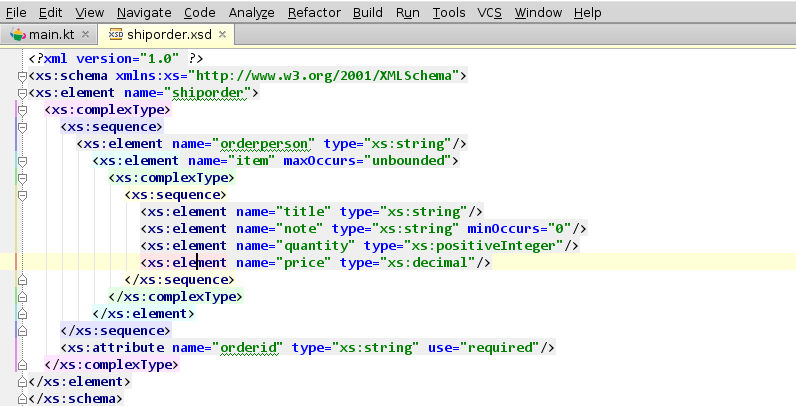
\includegraphics[height=4.132cm,width=8cm]{shiporder}

    {$\mathbf\downarrow$} % TODO: use tikz fot this: http://tex.stackexchange.com/questions/2152

    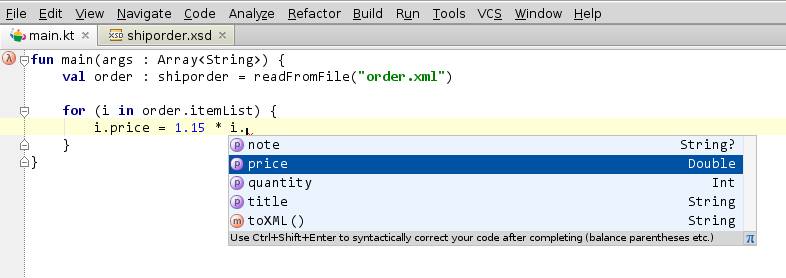
\includegraphics[height=2.829cm,width=8cm]{completion}
\end{center}
\end{frame}


\begin{frame}\frametitle{Качественные улучшения}
\linespread{1.1}
\begin{large}
    \begin{itemize}
        \item[---] Статические гарантии корректности
        \item[---] Согласованность с внешними интерфейсами
        \item[---] Упрощение рабочего процесса программиста
        \item[---] Отсутствие сгенерированных артефактов в системе контроля версий
    \end{itemize}
\end{large}
\linespread{1}
\end{frame}

\begin{frame}\frametitle{Количественные улучшения}
\begin{small}
\textbf{Уменьшение размера бинарной сборки:}
\begin{table}[!h]
    \begin{tabular}{ | l | c | c | c | c | }
    \hline
        & Кол-во типов & Программа & Удалено & Отношение \\ \hline
    Maven      & 166   & 4,5 Кб  & 684 Кб & 152 \\ \hline
    Facebook   & 599   & 15 Кб  & 2,5 Мб & 170 \\ \hline
    \end{tabular}
\end{table}

\textbf{Лаконичный код:}
\begin{table}[!h]
    \begin{tabular}{ | l | c | c | }
    \hline
    Язык    & Количество строк & Относительно Java \\ \hline
    Java    & 105   & 1 \\ \hline
    Gosu    & 36    & 0,34  \\ \hline
    Kotlin  & 41    & 0,39 \\
    \hline
    \end{tabular}
\end{table}

\end{small}
\end{frame}

\begin{frame}\frametitle{Заключение}
Реализованы механизмы загрузки типов для XML и языка C. \nl

\textbf{Результаты:}
    \begin{itemize}
        \item[---] Статические гарантии корректности
        \item[---] Уменьшение объема исходного кода и бинарной сборки
        \item[---] Упрощение рабочего процесса
    \end{itemize}
\end{frame}

\end{document}

% listing example
% \frame[containsverbatim]{
% \frametitle{Source code}

% \begin{lstlisting}[language=C]
% int main() {
%     printf("Hello World!");
%     return 0;
% }
% \end{lstlisting}
% }
